\documentclass[13pt]{article}

%% Language and font encodings
\usepackage[english]{babel}
\usepackage[utf8x]{inputenc}
\usepackage[T1]{fontenc}

%% Sets page size and margins
\usepackage[a4paper,top=2cm,bottom=2cm,left=1.5cm,right=1.5cm,marginparwidth=1.75cm]{geometry}

%% Useful packages
\usepackage{amsmath}
\usepackage{graphicx}
\usepackage[colorlinks=true, allcolors=blue]{hyperref}
\usepackage{parskip}
\usepackage{subfig}




\title{\vspace{-2.0cm}Bayesian Spatio-Temporal approach to weather forecasting\vspace{-2ex}}
\author{\vspace{-5.0cm}Adam Pluck\vspace{-3ex}}
\date{\vspace{-2ex}}



\begin{document}

\maketitle



Project Outline:

The aim of the project is to develop forecasting models for precipitation levels for future days. 


ever rising threat blah blah blah, hence why it is important to have good models for weather blah blah blah


Classical weather forecasting methods generally consist of numerical weather prediction (NWP). This is the way in which computer simulations, in conjunction with sophisticated mathematical and physical models use the oceans and atmosphere to predict future weather conditions. These models do, however, come with an ever increasing complexity. Even with the most powerful supercomputers, "forecast skill" drops off after just the 6th day. These models are also fundamentally flawed by their intrinsic sensitivity and underlying chaotic nature further reducing efficacy as they produce further in time forecasts.

One way to overcome this to take a data driven approach using machine learning techniques. This methodology is in its infancy when it comes to weather forecasting. Large meteorological entities such as the MetOffice are, however, exploring methods such as pure Gaussian Process regression or a hybrid of both GP and NWP. These methods generally forecast for each city or region, assuming independence between each city. Although this is done with some success, particularly exceeding in the long term (6days +) forecasts, it could be argued that we are losing accuracy from that assumption. Weather features between cities are most likely correlated in some way. Hence I aim to explore the idea of taking a Bayesian Spatio-Temporal approach to weather forecasting, utilising both trends in timeseries data of different weather features and also correlation in space between different locations of the United Kingdom. The ultimate goal is to produce a model that predicts precipitation in a given city.







\begin{center}
    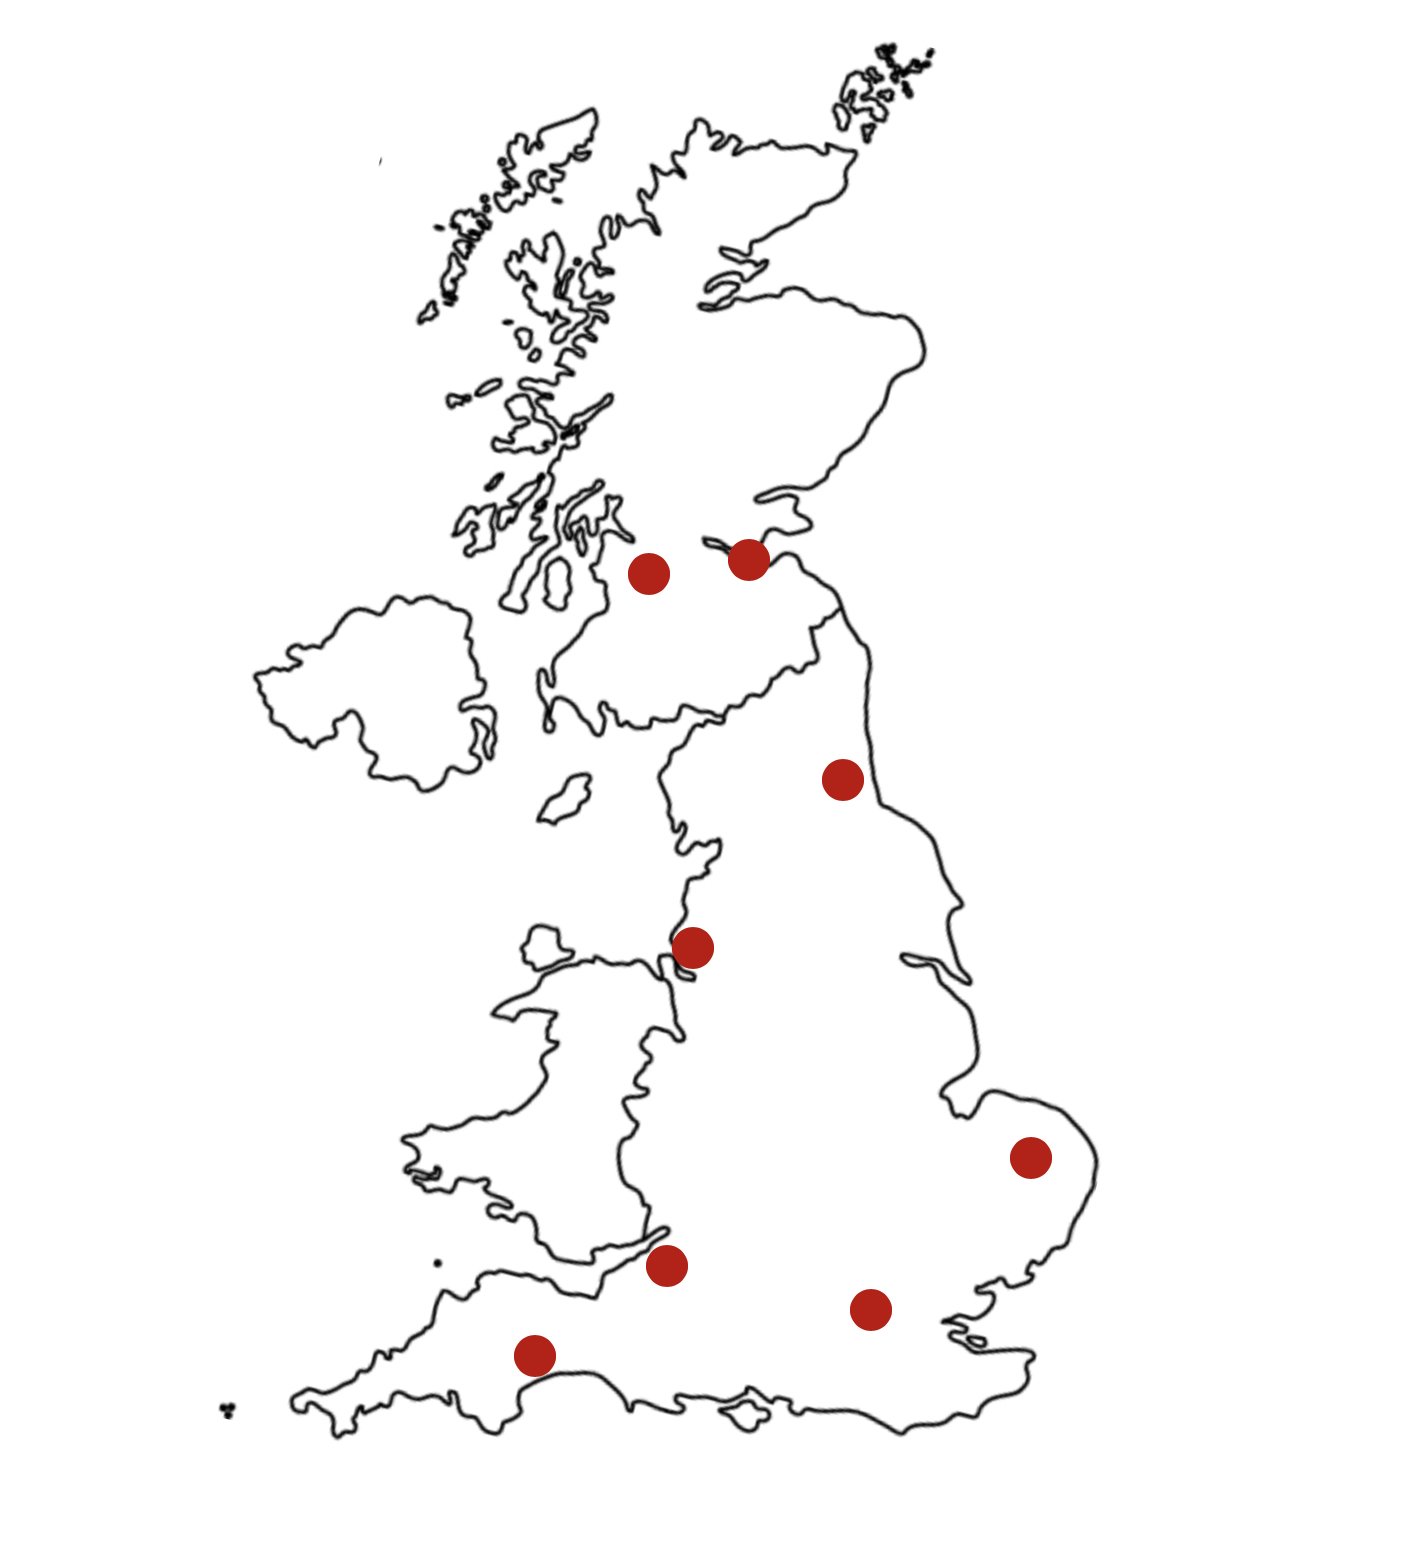
\includegraphics[width=70mm, scale=0.5]{images/ukMap.png}    
\end{center}

(Edinburgh, Glasgow, Newcastle, Liverpool, Norwich, Bristol, London, Exeter)



Project Plan:


Preface about the impact of weather on different departments (economy, agriculture, transport...) MAYBE 1 PAGEish


Talk about classic weather forecasting methods 1 Page

Talk about machine learning re forecasting 

Talk about how spatio-temporal forecasting may work 1 page


ACTUAL PROJECT:

Data collection, processing, feature selection


ACTUAL PREDICTION MAKING THING








Paper 1 - "A Probabilistic Approach for Weather Forecast using Spatio-temporal Inter-relationships among Climate Variables"







\end{document}